% 2026-10-23：按学习复现、探索尝试、优化验证、迭代调试、整板尝试重组。
\documentclass[stage2,fontset=fandol]{ydzjreport}
\usepackage{subcaption,longtable}

\stagetwosetup
{第 4 个逻辑月 · 迭代与调试}
{冯旭东、陈思文、张昊洋}
{复合微通道分区冷却}
{【待确认】逻辑月 4 对应的自然月}
{小块分界线；结构复杂性；Bi；扰流柱数量；XGBoost 待开展}
{探究不同热流密度下小块选择的适用边界，围绕 Bi 与扰流柱数量迭代理论，并准备基于翼型参数分组的 XGBoost 尝试。}
\pagestyle{empty}   % 去掉页眉与页脚（含页码）

\begin{document}
\makestagetwohead

% unified-five-part-outline 2026-10-23
\section{本月计划}

\subsection{任务目标}

本月从多种结构的探索结果回到小块理论，研究不同热流密度下应该选哪一种小块，以及选择何时发生变化。此处的分界线是小块适用范围，不是逻辑月三的翼型参数分组。代理模型拟承接月三分组，但 XGBoost 尚未开展。

\section{研究过程}

\subsection{文献与理论准备}

\subsubsection{本阶段文献与资料}

本月承接月二的结构探索、月三的翼型参数方案和数值核验，以及已有代理模型方法资料。Bi 与扰流柱数量部分目前缺少归档的专门计算记录，以下仅给出分析框架和需补证据。

\subsubsection{对本方向的启示}

结构形状、换热面积、扰流柱数量和水力阻力会共同改变温度表现。因此不能把“结构复杂”直接当作性能优势，也不能只按热流密度给出脱离流量、温度上限及泵功约束的固定选择。



\subsection{研究步骤与分析框架}

\subsubsection{由探索结果提出小块选择分界线问题}
已有常规、仿生和翼型结构结果显示温度收益与水力代价需要联合评价。例如月二保存记录中，300 W/cm$^2$下直线、正弦和 NACA2416 的最高温度分别为52.50、62.27和72.48 $^\circ$C，水力功率分别为0.04919、0.05897和0.01566 W。三者运行条件并非等泵功对照，不能据这些值直接确定适用分界线；这些记录的作用是提出“在什么约束下选哪一种小块”的问题。

\subsubsection{分界线的研究设计}
拟在统一几何尺度、入口条件和物性下扫描热流密度，先排除超出温度或压降限制的结构，再在满足限制的候选中比较泵送代价或统一综合指标。相同流量与相同泵功属于不同的比较方式，应分别报告。分界线可能随约束改变，也可能出现重叠可选区或没有可行结构的区间，不预先假设唯一阈值。

【待补：候选小块清单、扫描范围、约束值、性能曲线及分界线不确定性。】

\subsubsection{Bi 验证思路与小块理论边界}
本稿将 Bi 作为待验证的尺度分析工具。若采用常见固体导热与对流比较形式，需明确
\begin{equation}
Bi=\frac{hL_c}{k_s},\qquad L_c=\frac{V_s}{A_{\mathrm{conv}}}.
\label{eq:bi}
\end{equation}
式~\eqref{eq:bi} 中 $k_s$ 为固体导热系数，$V_s$ 为声明的固体体积，$A_{\mathrm{conv}}$ 为相应对流面积，$h$ 应注明提取位置与平均方式。这是建议采用的定义，实际尺度与统计区域仍需结合小块模型确认。Bi 可辅助讨论内部导热与表面对流的相对影响；相邻小块的横向导热耦合还需温度场或热量分配对照，不能由一个 Bi 值直接证明独立小块假设成立。

【待补：实际 Bi 定义、各结构计算表、与温度场的一致性验证。】

\subsubsection{扰流柱数量影响的迭代分析}
本月研究重点是扰流柱数量在换热中的作用。数量改变会同时影响固液面积、流通截面、阻塞及柱间干扰，因此需要与翼型形状效应区分。拟固定外形尺寸、单柱几何和边界条件，改变柱数并记录排列、间距和总面积，联合比较最高温度、换热量、压降与水力功率；必要时再用等面积对照辨识数量与面积的影响。

目前尚未归档支持数量效应大小的完整对照数据，不给出“增加多少柱即提高多少换热”的结论。
【待补：柱数、排列、换热面积和对应性能数据。】

\subsubsection{基于翼型参数分组的 XGBoost 准备}
XGBoost 尚未开展。拟先核对月三参数组，将厚度、弯度、攻角及可用工况作为候选输入，选择定义统一的温度或压降指标作为输出，再建立基础回归和 XGBoost 对照。参数组没有数据时不能直接开始训练；已有13条分支混含物性、网格和时刻变化，也不能未经筛选当作13个独立合格训练样本。

后续需按几何或工况组合划分训练与测试，避免同一算例的近邻或重复记录跨集合，并报告误差、范围和训练成本。当前不填模型精度、泛化或加速收益。

\section{完成情况}

\subsection{任务完成状态}

\begin{table}[H]\centering
\caption{本月工作与材料状态}\label{tab:tasks}
\begin{tabularx}{\textwidth}{@{}Y Y Y@{}}
\toprule
\rowcolor{ydzjlight} 工作 & 状态 & 依据或缺口 \\
\midrule
小块适用分界线 & 研究问题已明确 & 尚缺统一约束下的扫描数据和交界热流密度 \\
复杂性与性能关系 & 已有探索依据 & 现有记录可提示问题，尚不能给出通用排序 \\
Bi 验证 & 待补依据 & 需给出特征尺度、物性、换热系数及计算结果 \\
扰流柱数量影响 & 研究重点已明确 & 需数量对照和换热、水力指标支持定量判断 \\
翼型 XGBoost & 尚未开展 & 待月三分组数据补齐后训练和测试 \\
\bottomrule\end{tabularx}\end{table}

\subsection{关键结果与完成边界}

本月已明确小块适用分界线、Bi 验证、数量效应和代理模型四项研究任务。Bi 验证结论或 XGBoost 预测结果，保留为待补项。

\subsection{四种流道的温度表现与适用热流密度区间}

把四种流道各自的 39 个有效工况按热流密度连成曲线（图~\ref{fig:month4-trend}），
数据由 Case／Data 文件逐点提取。同一流道内各点只改变热流密度，
入口温度与入口速度不变；不同流道之间不共享同一热负荷序列。

\begin{figure}[htbp]
\centering
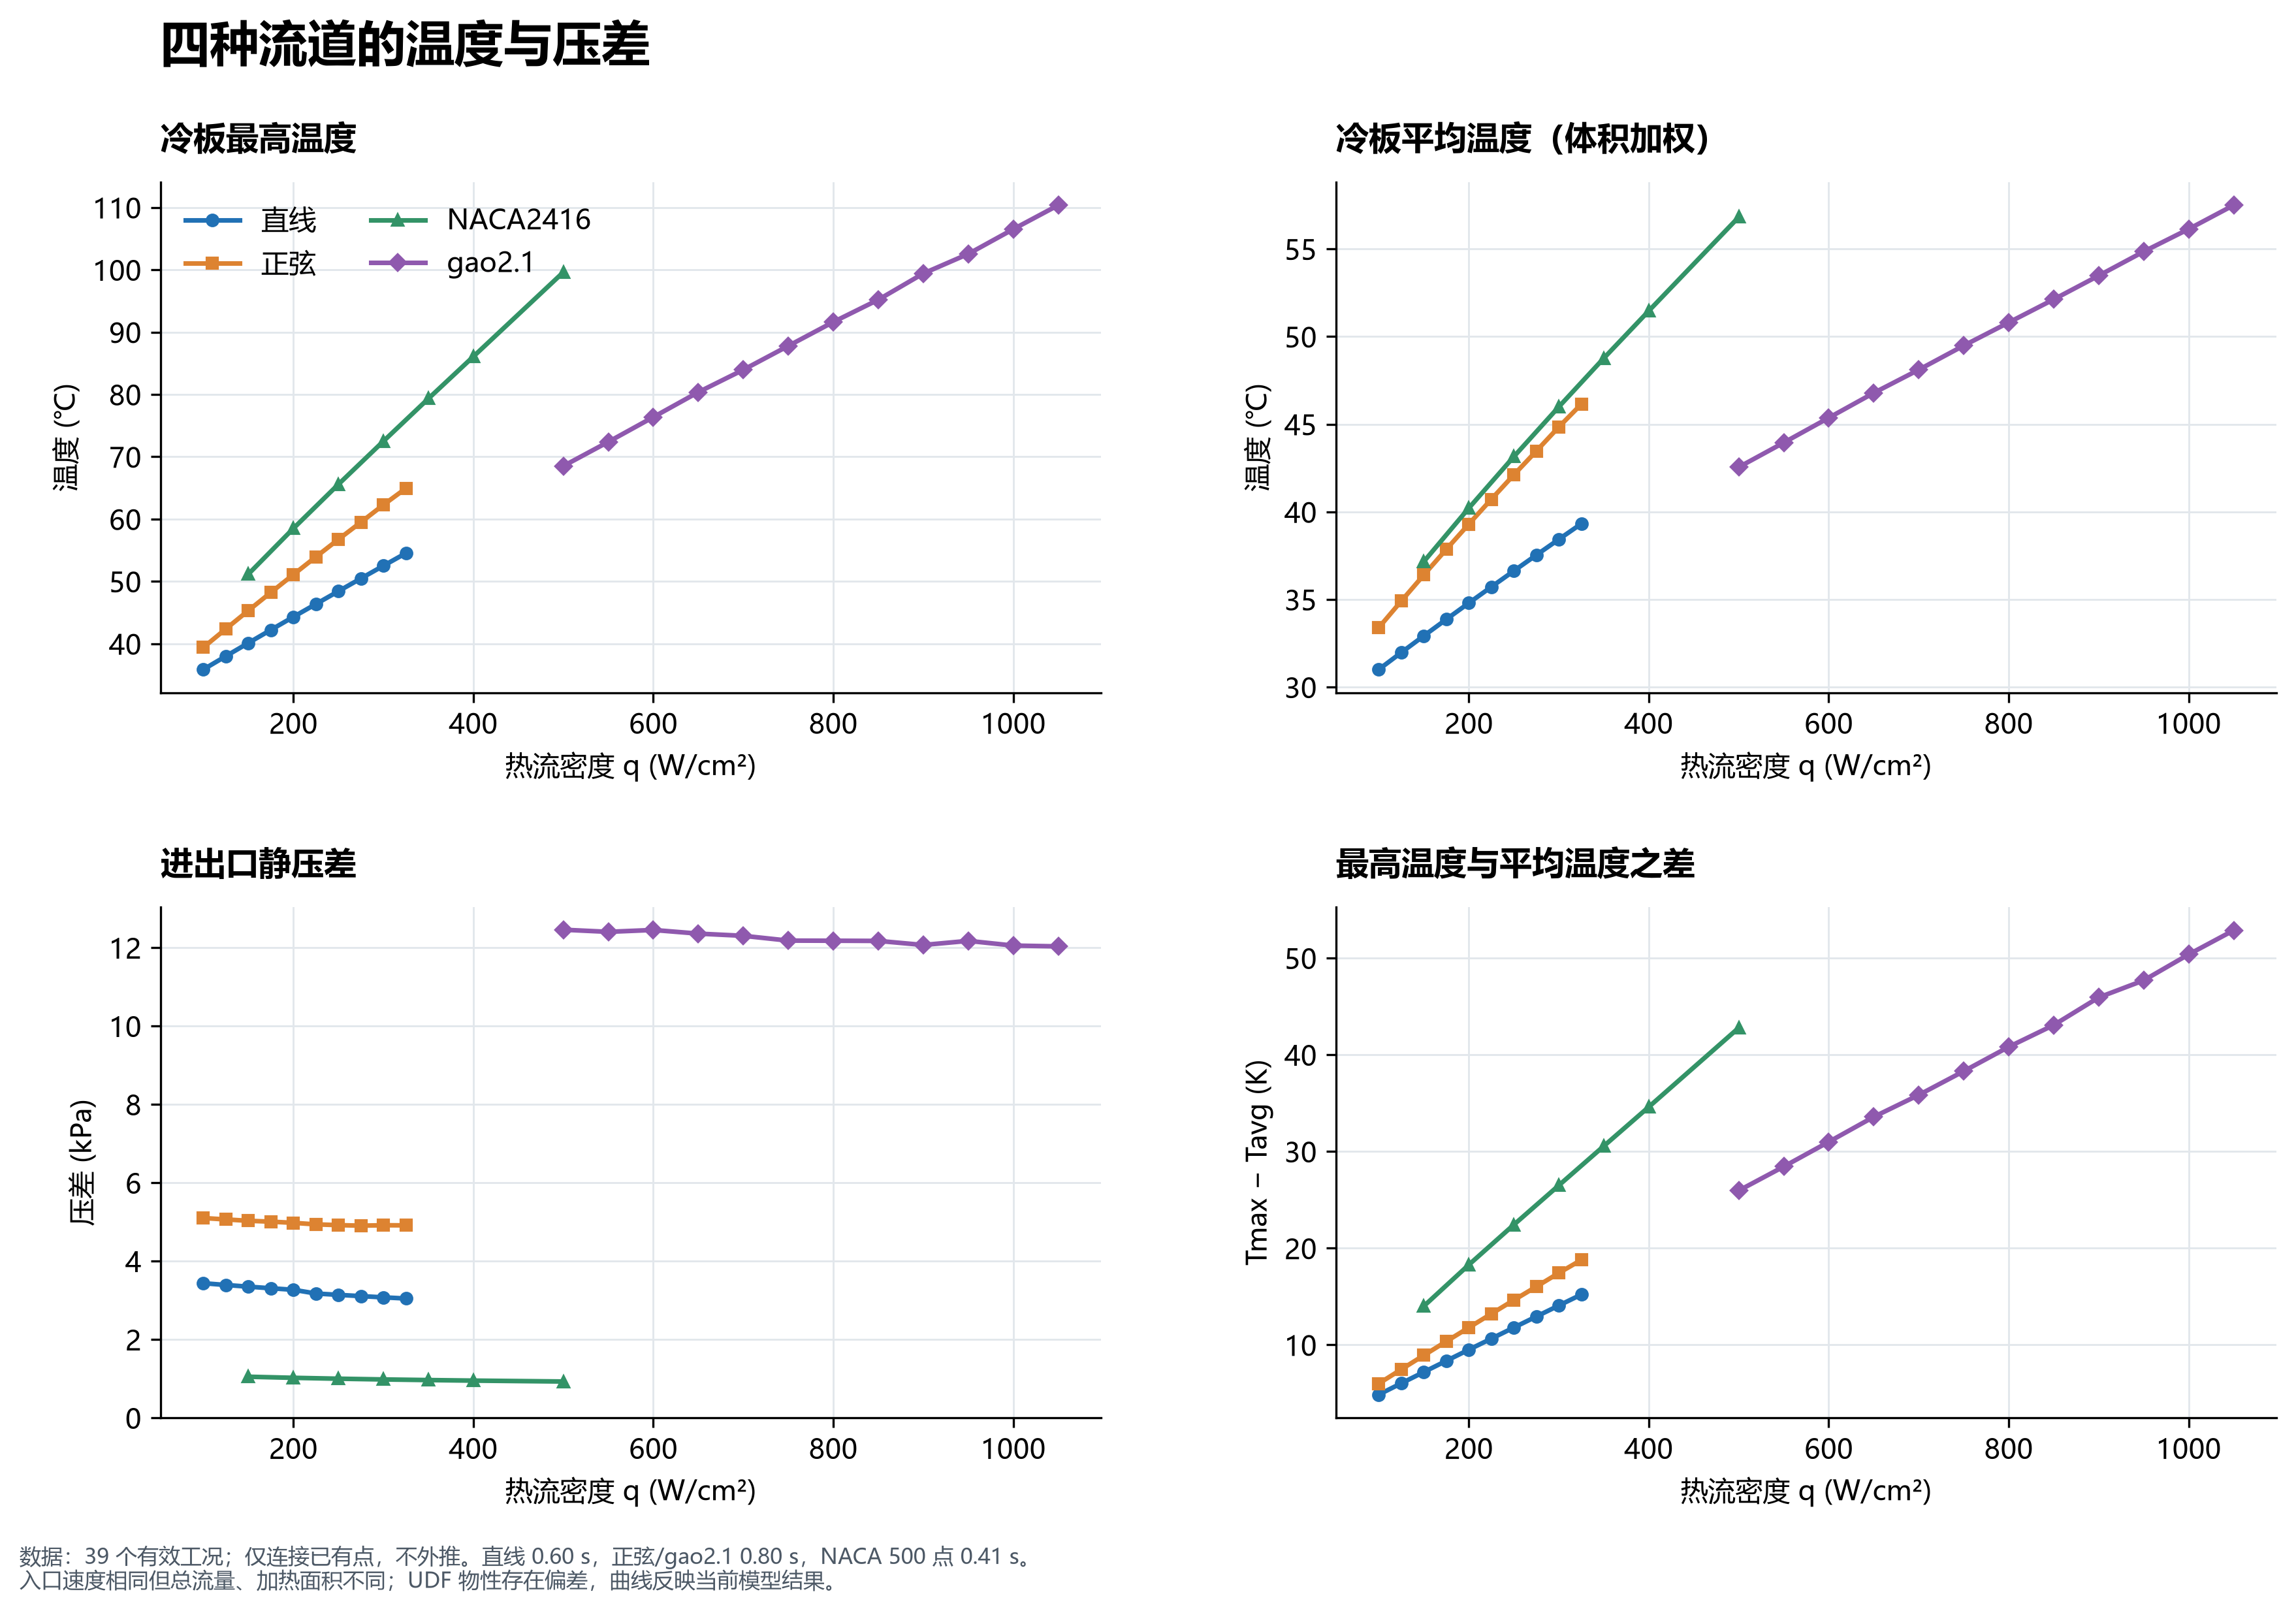
\includegraphics[width=\textwidth]{figs/30_四流道总览.png}
\caption{四种流道的最高温度、体积平均温度、进出口静压差与峰值—平均温差随热流密度的变化。仅连接已算点，不插值外推；gao2.1 从 500 W/cm$^2$ 起，直线与正弦止于 325 W/cm$^2$。}
\label{fig:month4-trend}
\end{figure}

随热流密度增加，四种流道的冷板最高温度、体积平均温度与峰值偏离平均值同步上升，
最高温度用于识别热端约束，体均温度反映总体热状态。
在整个已算区间内，
最高温度始终是直线最低、正弦次之、NACA2416 再次、gao2.1 最高；
压差与水力功率则始终是 NACA2416 最低、直线次之、正弦再次、gao2.1 最高。
这说明温度与水力代价的排序不随热流密度改变，改变的是各方案可用的区间。

\par\needspace{8\baselineskip}

\FloatBarrier
\begin{table}[H]\centering\small
\caption{四种流道的工况与几何核对}\label{tab:month4-conditions}
\begin{tabularx}{\textwidth}{@{}l c c c c c@{}}
\toprule
\rowcolor{ydzjlight} 流道 & $q$ 范围 & 总入口面积 & 流量 & 加热面积 & 保存时刻 \\
 & / (W/cm$^2$) & / mm$^2$ & / (L/min) & / cm$^2$ & / s \\
\midrule
直线     & 100--325  & 8.00 & 0.96 & 0.1050 & 0.60 \\
正弦     & 100--325  & 6.00 & 0.72 & 0.1225 & 0.80 \\
NACA2416 & 150--500  & 8.00 & 0.96 & 0.1225 & 0.80\\
gao2.1   & 500--1050 & 4.50 & 0.54 & 0.1225 & 0.80 \\
\bottomrule
\end{tabularx}
\end{table}

四种方案的入口速度均为 2 m/s、入口温度均为 300 K。


\begin{figure}[htbp]
\centering
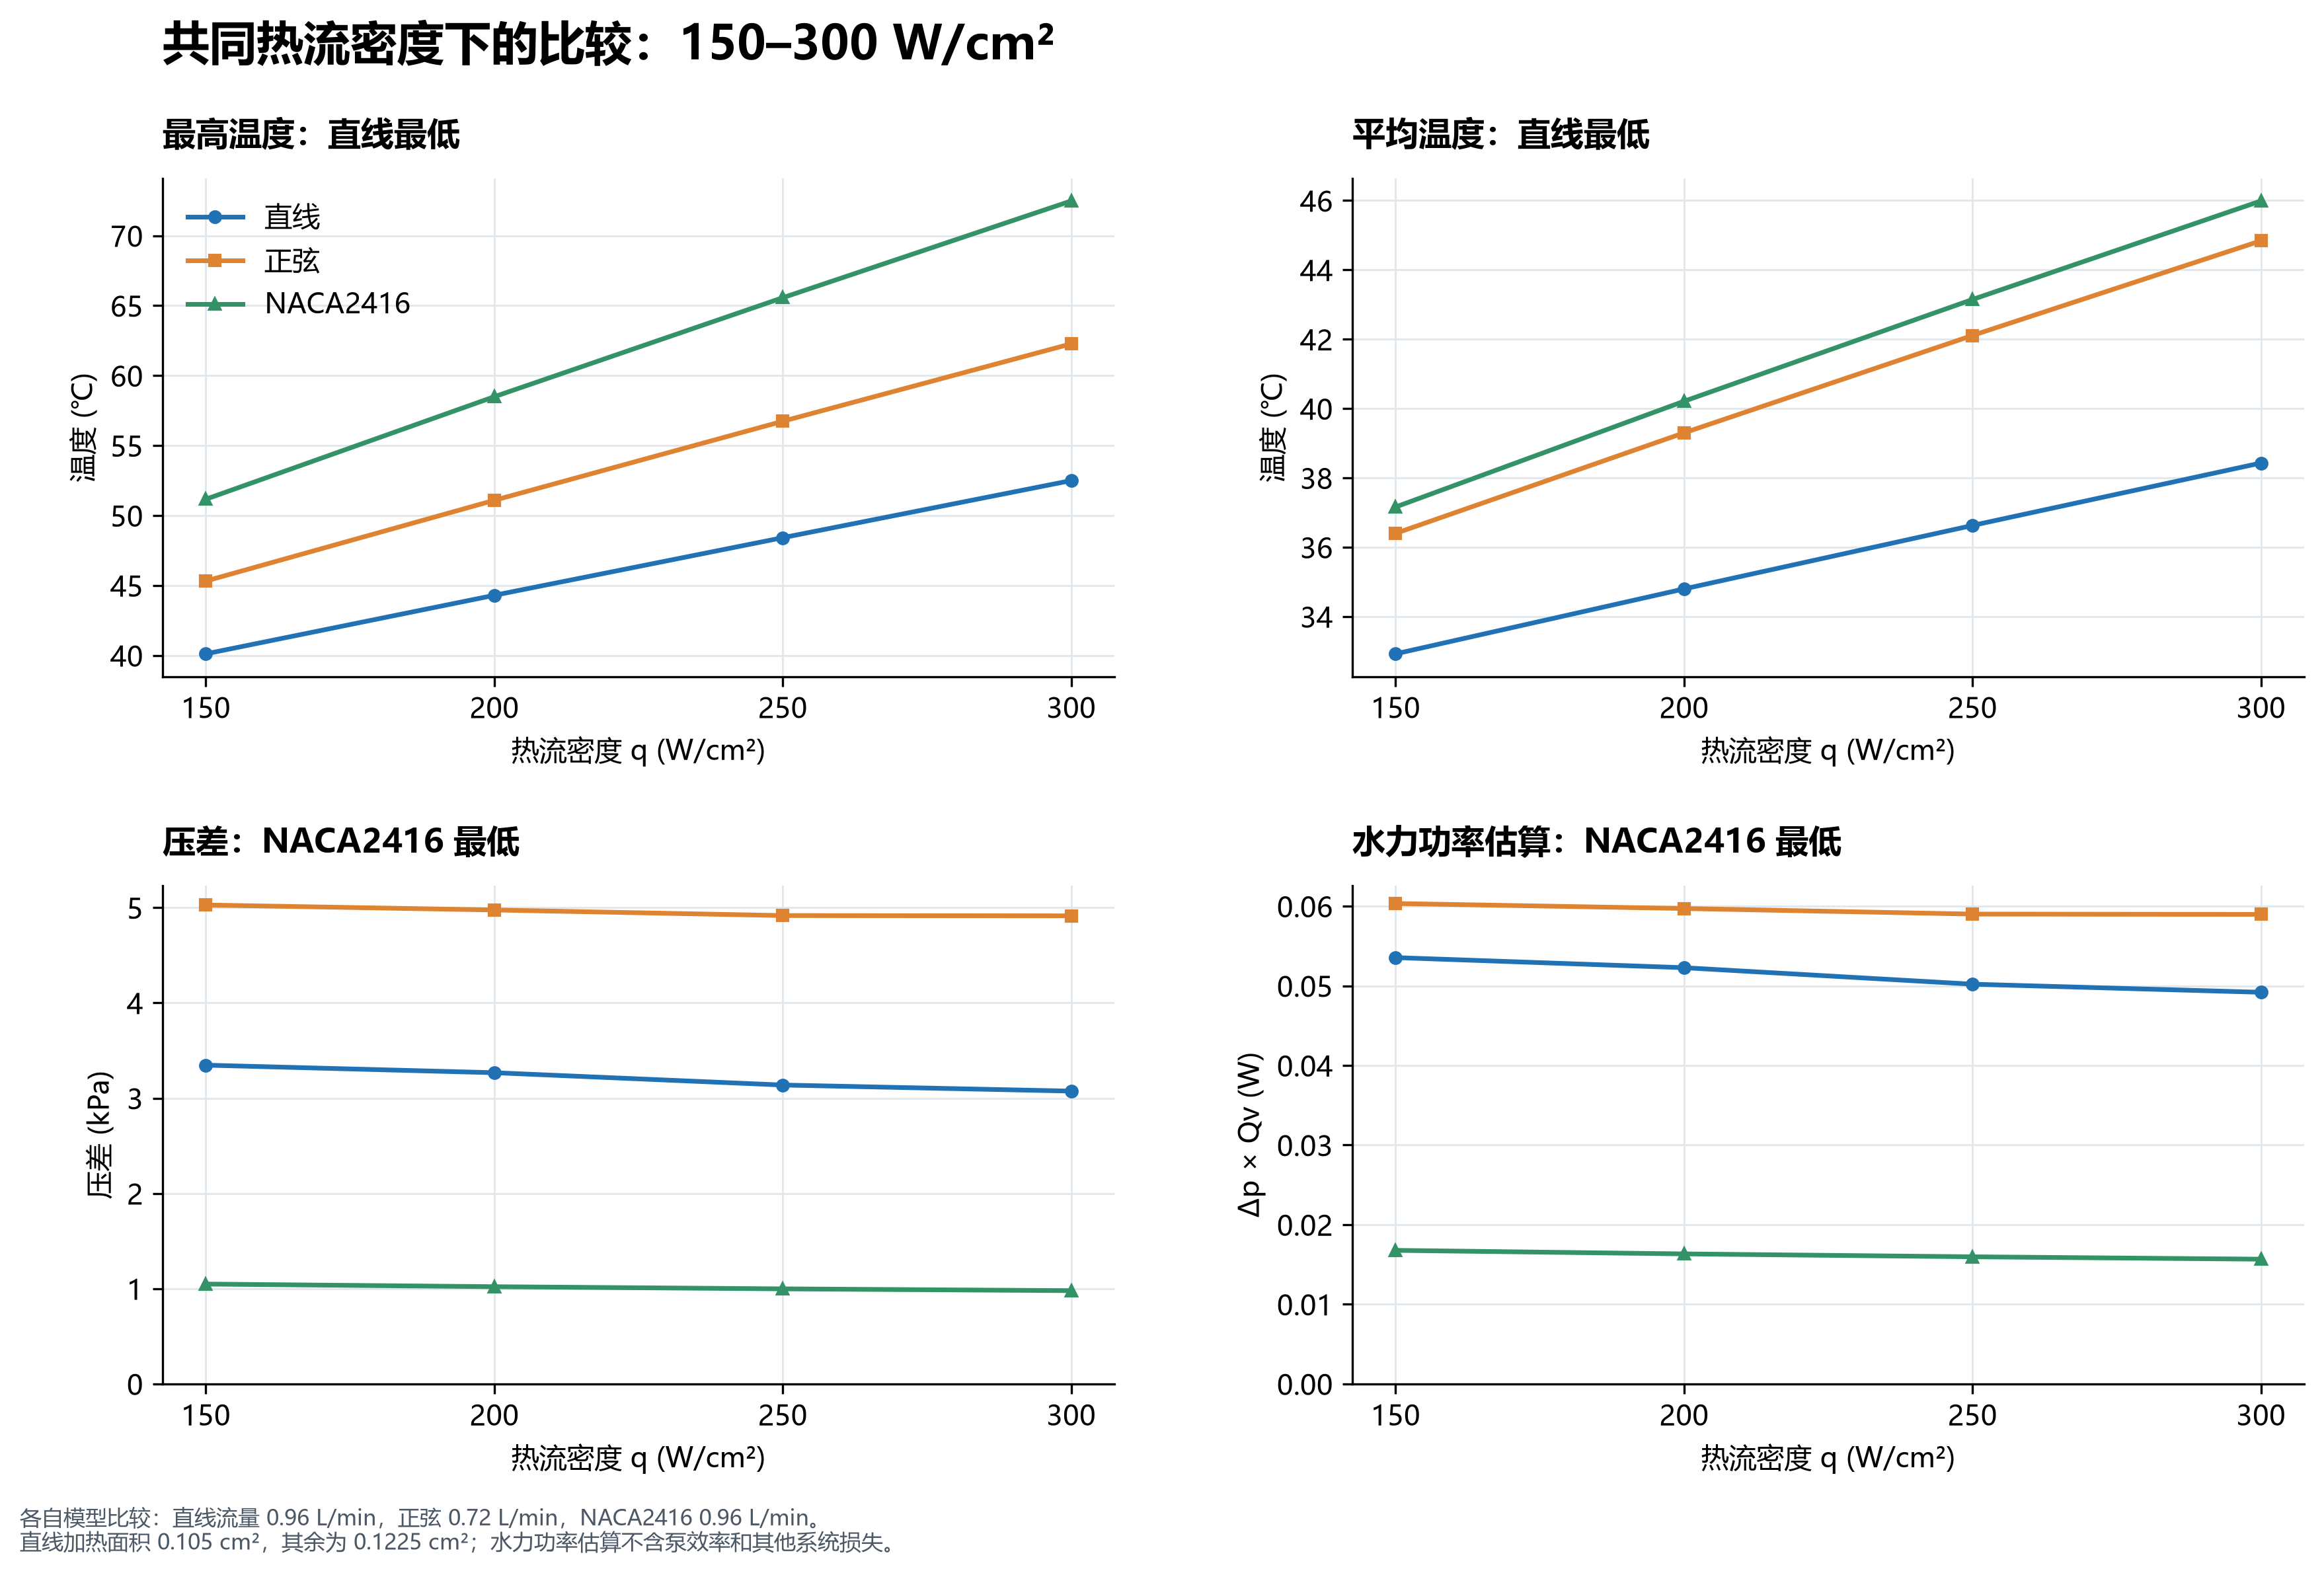
\includegraphics[width=\textwidth]{figs/31_共同热流密度比较.png}
\caption{150、200、250、300 W/cm$^2$ 四个共同数据点上的比较：最高温度、体积平均温度、压差与水力功率估算。}
\label{fig:month4-common}
\end{figure}

图~\ref{fig:month4-common} 给出三方案共同算过的 150--300 W/cm$^2$ 区间。
最高温度与体均温度的次序为直线 $<$ 正弦 $<$ NACA2416，
压差与水力功率的次序为 NACA2416 $<$ 直线 $<$ 正弦；
300 W/cm$^2$ 时直线最高温度 52.50 $^\circ$C，正弦 62.27 $^\circ$C（高 9.77 $^\circ$C），
NACA2416 72.48 $^\circ$C（高 19.98 $^\circ$C）。
三者的最高温度都在 80 $^\circ$C 以内，温度均有余量，
因此该区间的取舍主要取决于泵送代价：
\textbf{直线与正弦在温度上占优，NACA2416 在压降上占优。}

\FloatBarrier
\begin{table}[H]\centering
\caption{四种流道的适用区间与依据}\label{tab:month4-advice}
\begin{tabularx}{\textwidth}{@{}l Y Y@{}}
\toprule
\rowcolor{ydzjlight} 流道 & 适用区间与定位 & 数据依据 \\
\midrule
直线 & 中低热流密度，温度优先 & 100--325 W/cm$^2$；共同区间内最高温度、平均温度均最低，压差与水力功率低于正弦 \\
正弦 & 中低热流密度，与直线同档 & 100--325 W/cm$^2$；温度略高于直线、压差与水力功率略高，仍低于 NACA2416 的温度水平 \\
NACA2416 & 中低热流密度，压降优先 & 150--500 W/cm$^2$；共同区间内压差与水力功率最低，为直线的 31.8\%、正弦的 19.9\%，300 W/cm$^2$ 时最高温度 72.5 $^\circ$C \\
gao2.1 & 高热流密度 & 500--1050 W/cm$^2$；500 点最高温度 68.50 $^\circ$C，1050 点 110.36 $^\circ$C，是唯一覆盖 1000 W/cm$^2$ 以上的方案 \\
\bottomrule
\end{tabularx}
\end{table}

表~\ref{tab:month4-advice} 把上述结果整理为三种定位：
中低热流密度下由直线与正弦承担温度控制，NACA2416 作为减压降方案，
500 W/cm$^2$ 以上交给 gao2.1。

\begin{figure}[htbp]
\centering
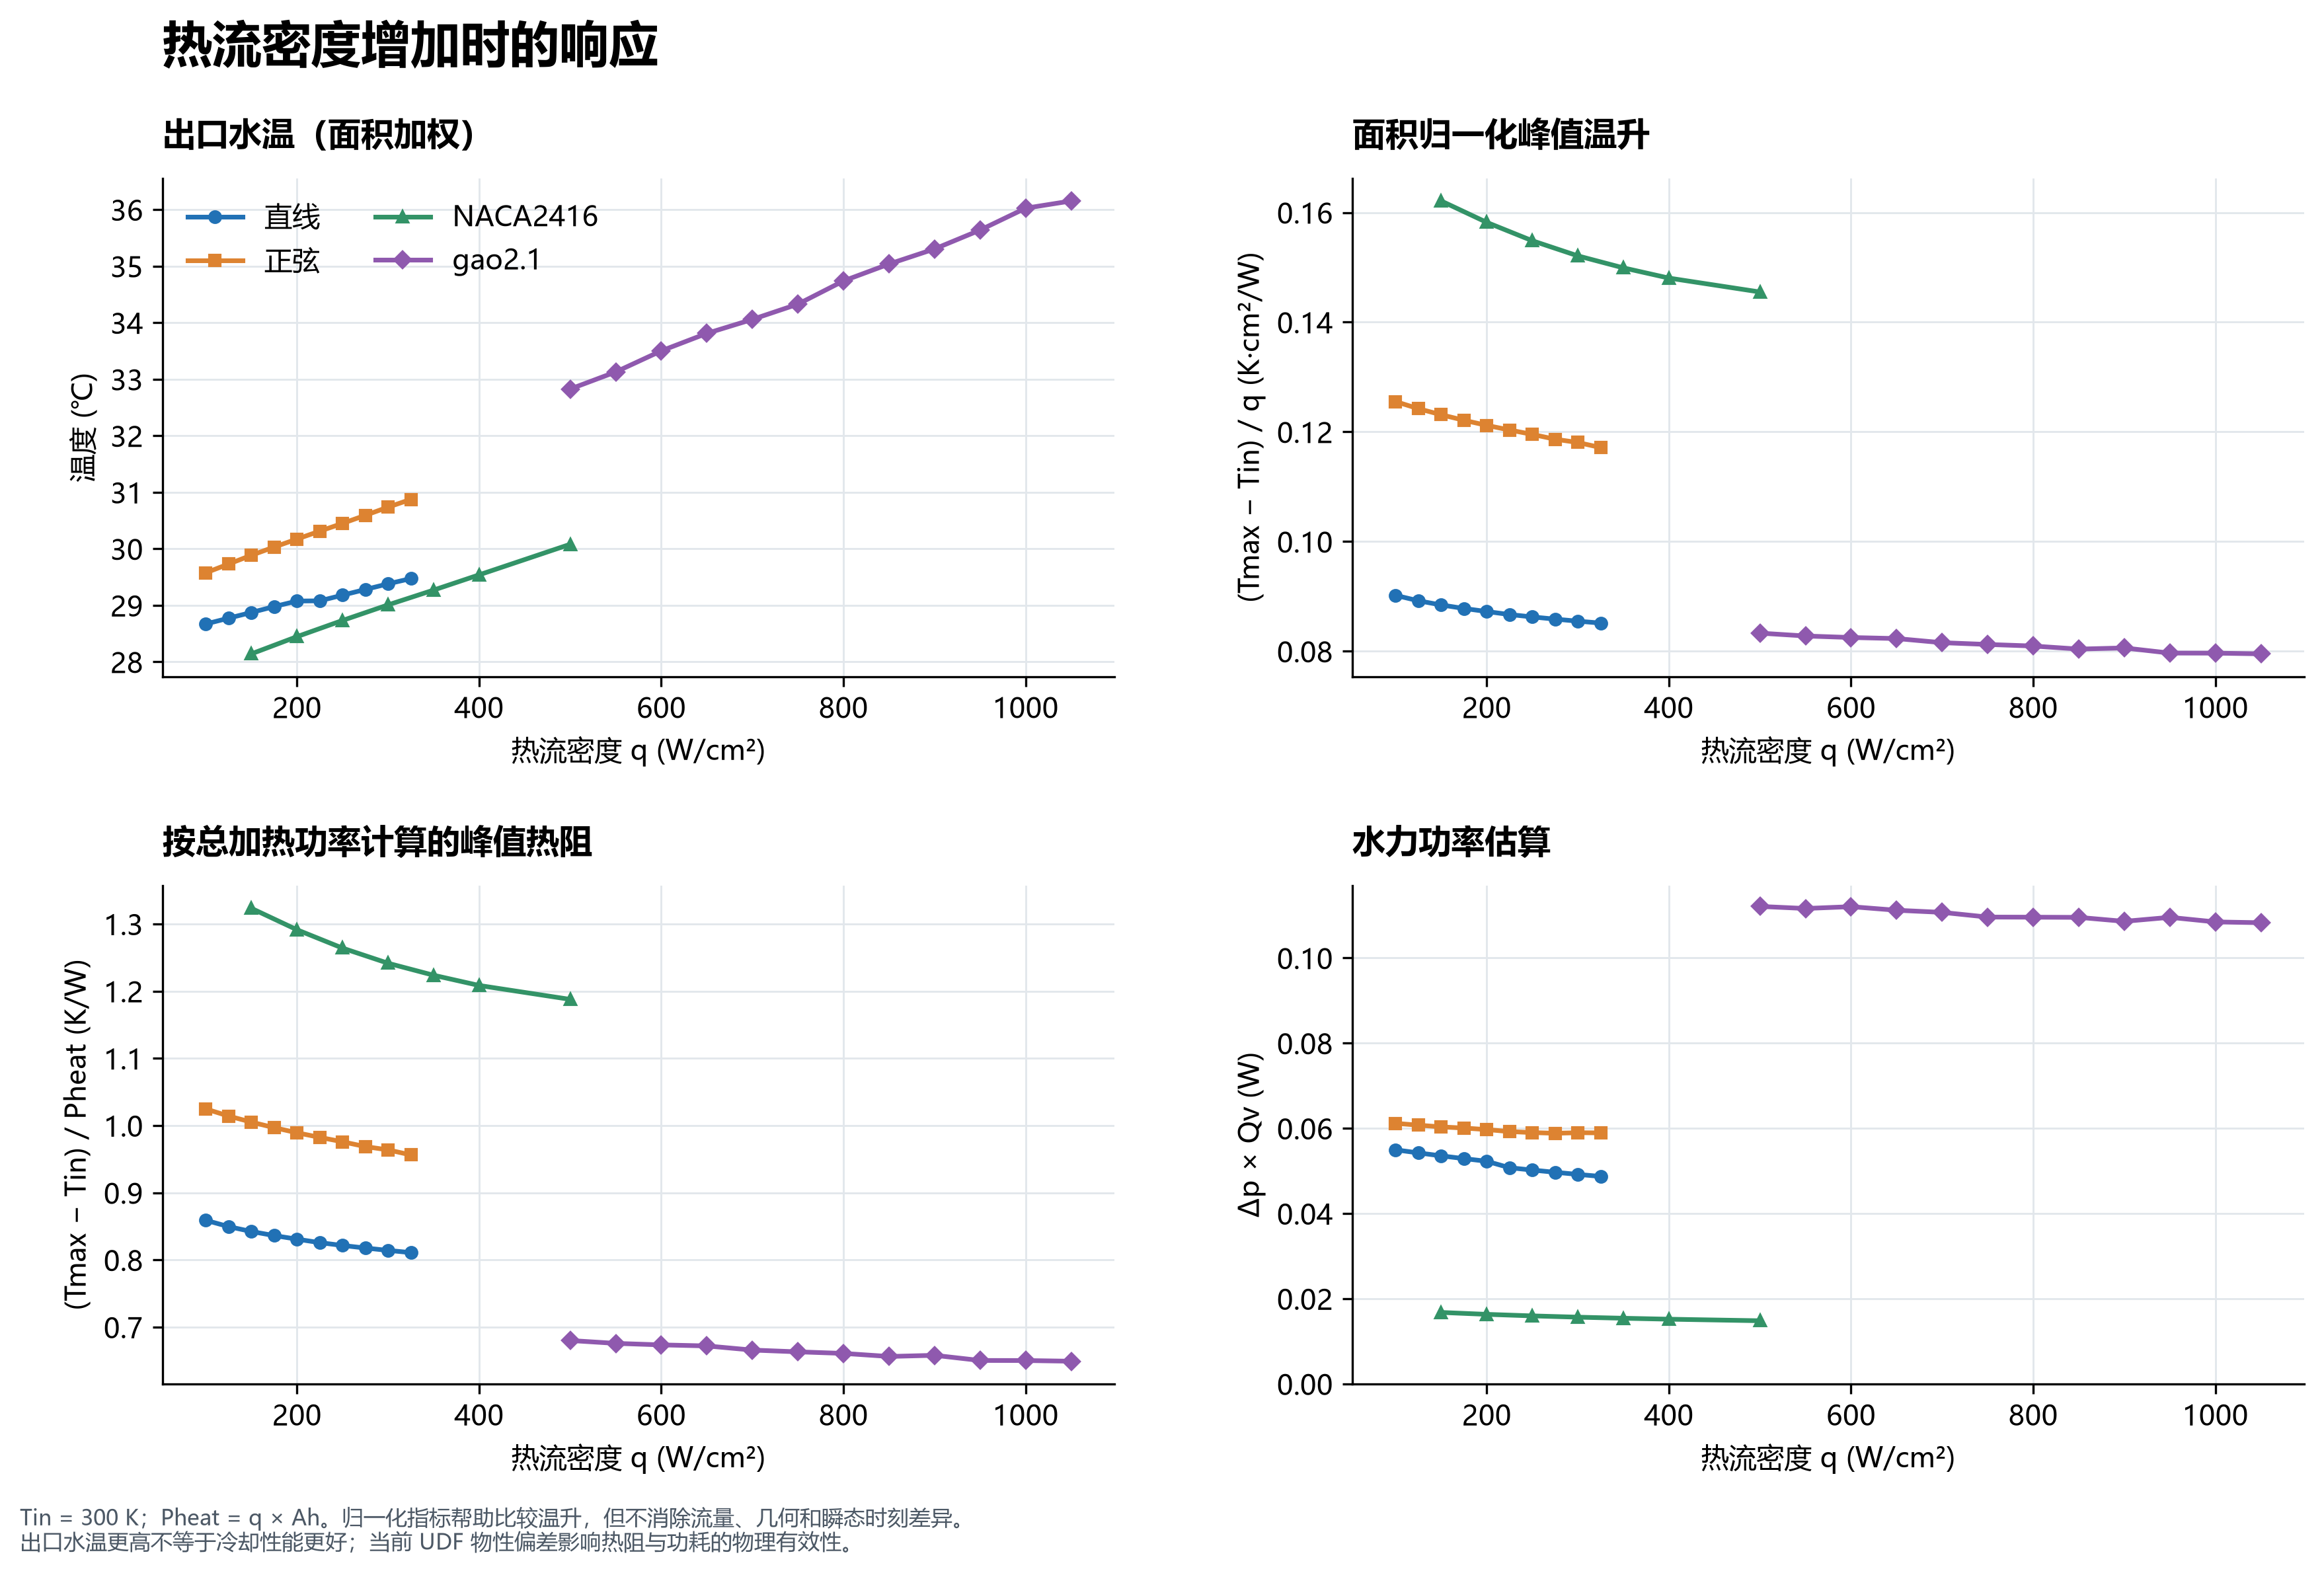
\includegraphics[width=\textwidth]{figs/32_归一化指标与水力代价.png}
\caption{出口水温、面积归一化峰值温升、按总加热功率计算的峰值热阻与水力功率估算随热流密度的变化。$R''_{\max}=(T_{\max}-T_{\mathrm{in}})/q$，$R_{\max}=(T_{\max}-T_{\mathrm{in}})/(qA_h)$，$P_{\mathrm{hyd}}=\Delta p\,Q_v$。}
\label{fig:month4-normalized}
\end{figure}

图~\ref{fig:month4-normalized} 把温度与压差折算成面积归一化温升 $R''_{\max}$、
峰值热阻 $R_{\max}$ 与水力功率估算 $P_{\mathrm{hyd}}$，结论与直接比较一致：
中低热流密度段直线的 $R''_{\max}$ 最低，NACA2416 的 $P_{\mathrm{hyd}}$ 最低；
到 500 点，gao2.1 的 $R_{\max}$ 为 0.680 K/W，低于 NACA2416 的 1.188 K/W，
但水力功率估算升至 0.11211 W，是 NACA2416（0.01482 W）的 7.57 倍，
压差则相差 13.45 倍——高热流密度段用更大的泵送代价换取温度上限。

\begin{figure}[htbp]
\centering
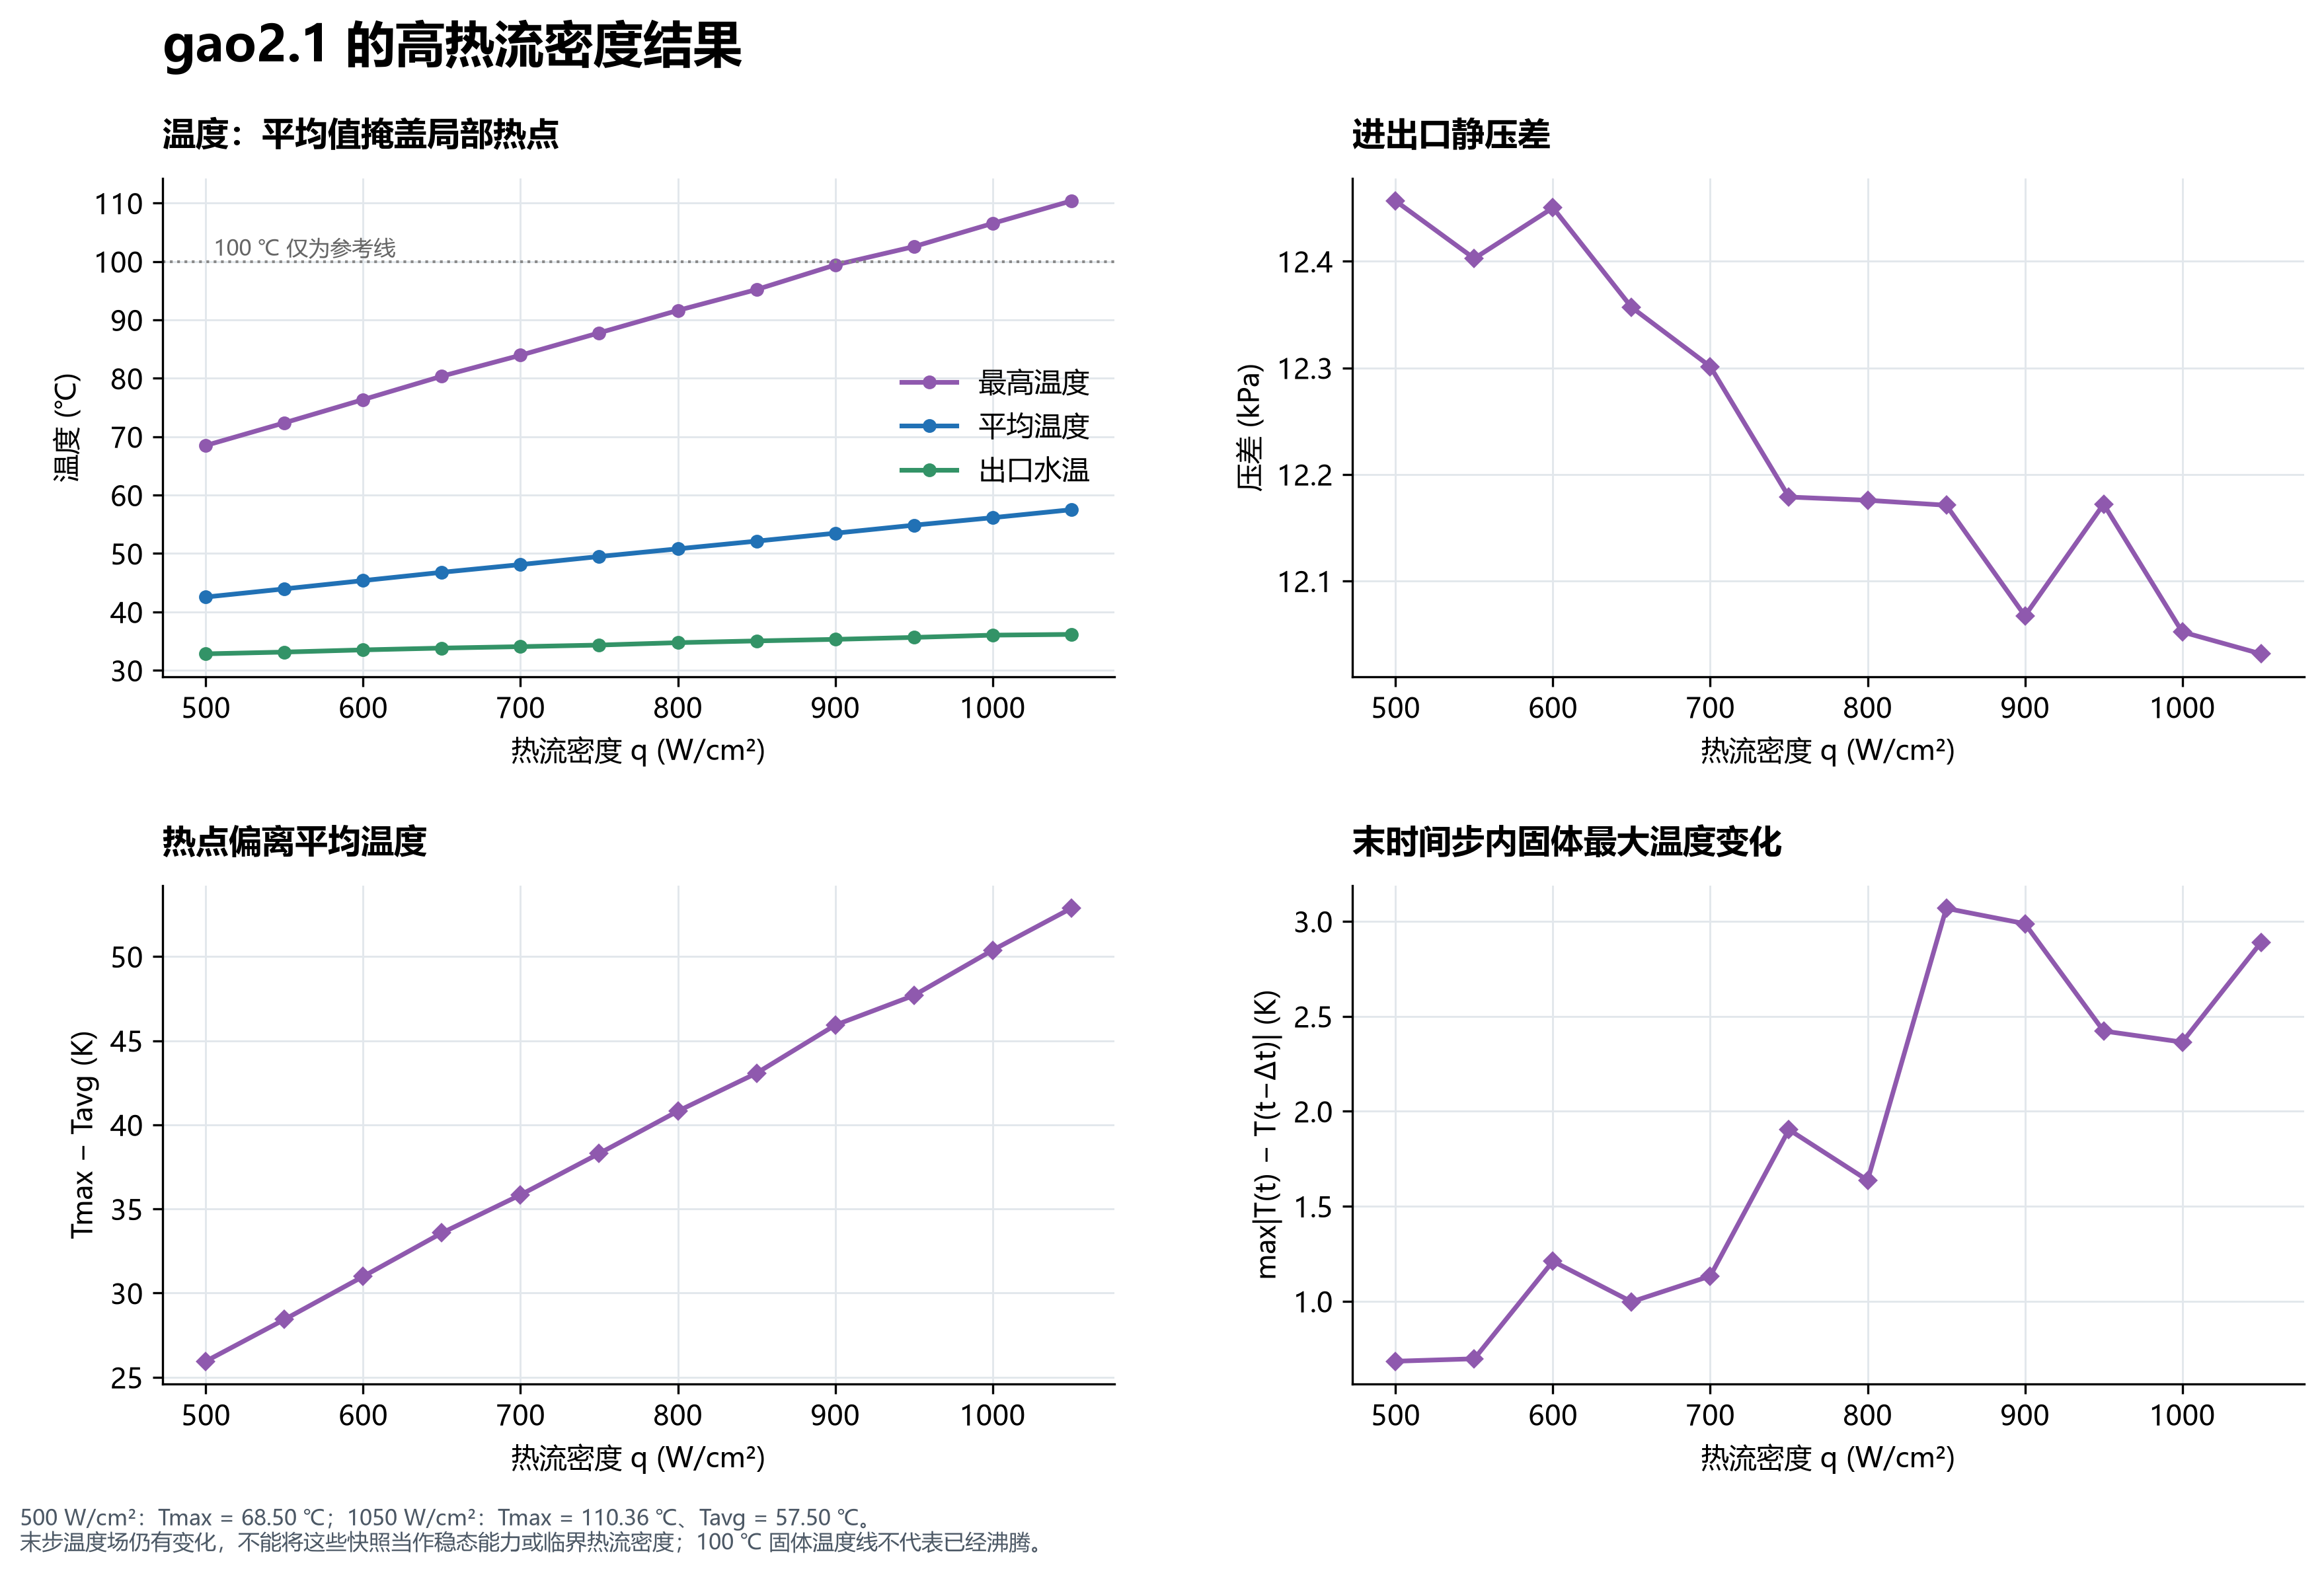
\includegraphics[width=\textwidth]{figs/33_gao2.1高热流密度.png}
\caption{gao2.1 在 500--1050 W/cm$^2$ 区间的温度、压差与末时间步温度变化。最高温度由 500 点的 68.50 $^\circ$C 升至 1050 点的 110.36 $^\circ$C，1050 点体积平均温度仅 57.50 $^\circ$C。}
\label{fig:month4-gao}
\end{figure}

gao2.1 是唯一覆盖 1000 W/cm$^2$ 以上的流道（图~\ref{fig:month4-gao}）。
其最高温度由 500 点的 68.50 $^\circ$C 升到 1050 点的 110.36 $^\circ$C，
体积平均温度只到 57.50 $^\circ$C，峰值与平均值相差 52.86 K，
热点集中在局部而不是整板过热。
按现有数据线性插值，80 $^\circ$C 温度上限对应 gao2.1 约 645.5 W/cm$^2$、
NACA2416 约 355.1 W/cm$^2$、正弦约 279.6 W/cm$^2$，
直线在已算的最高点 325 W/cm$^2$ 也只有 54.52 $^\circ$C。


\begin{figure}[htbp]
\centering
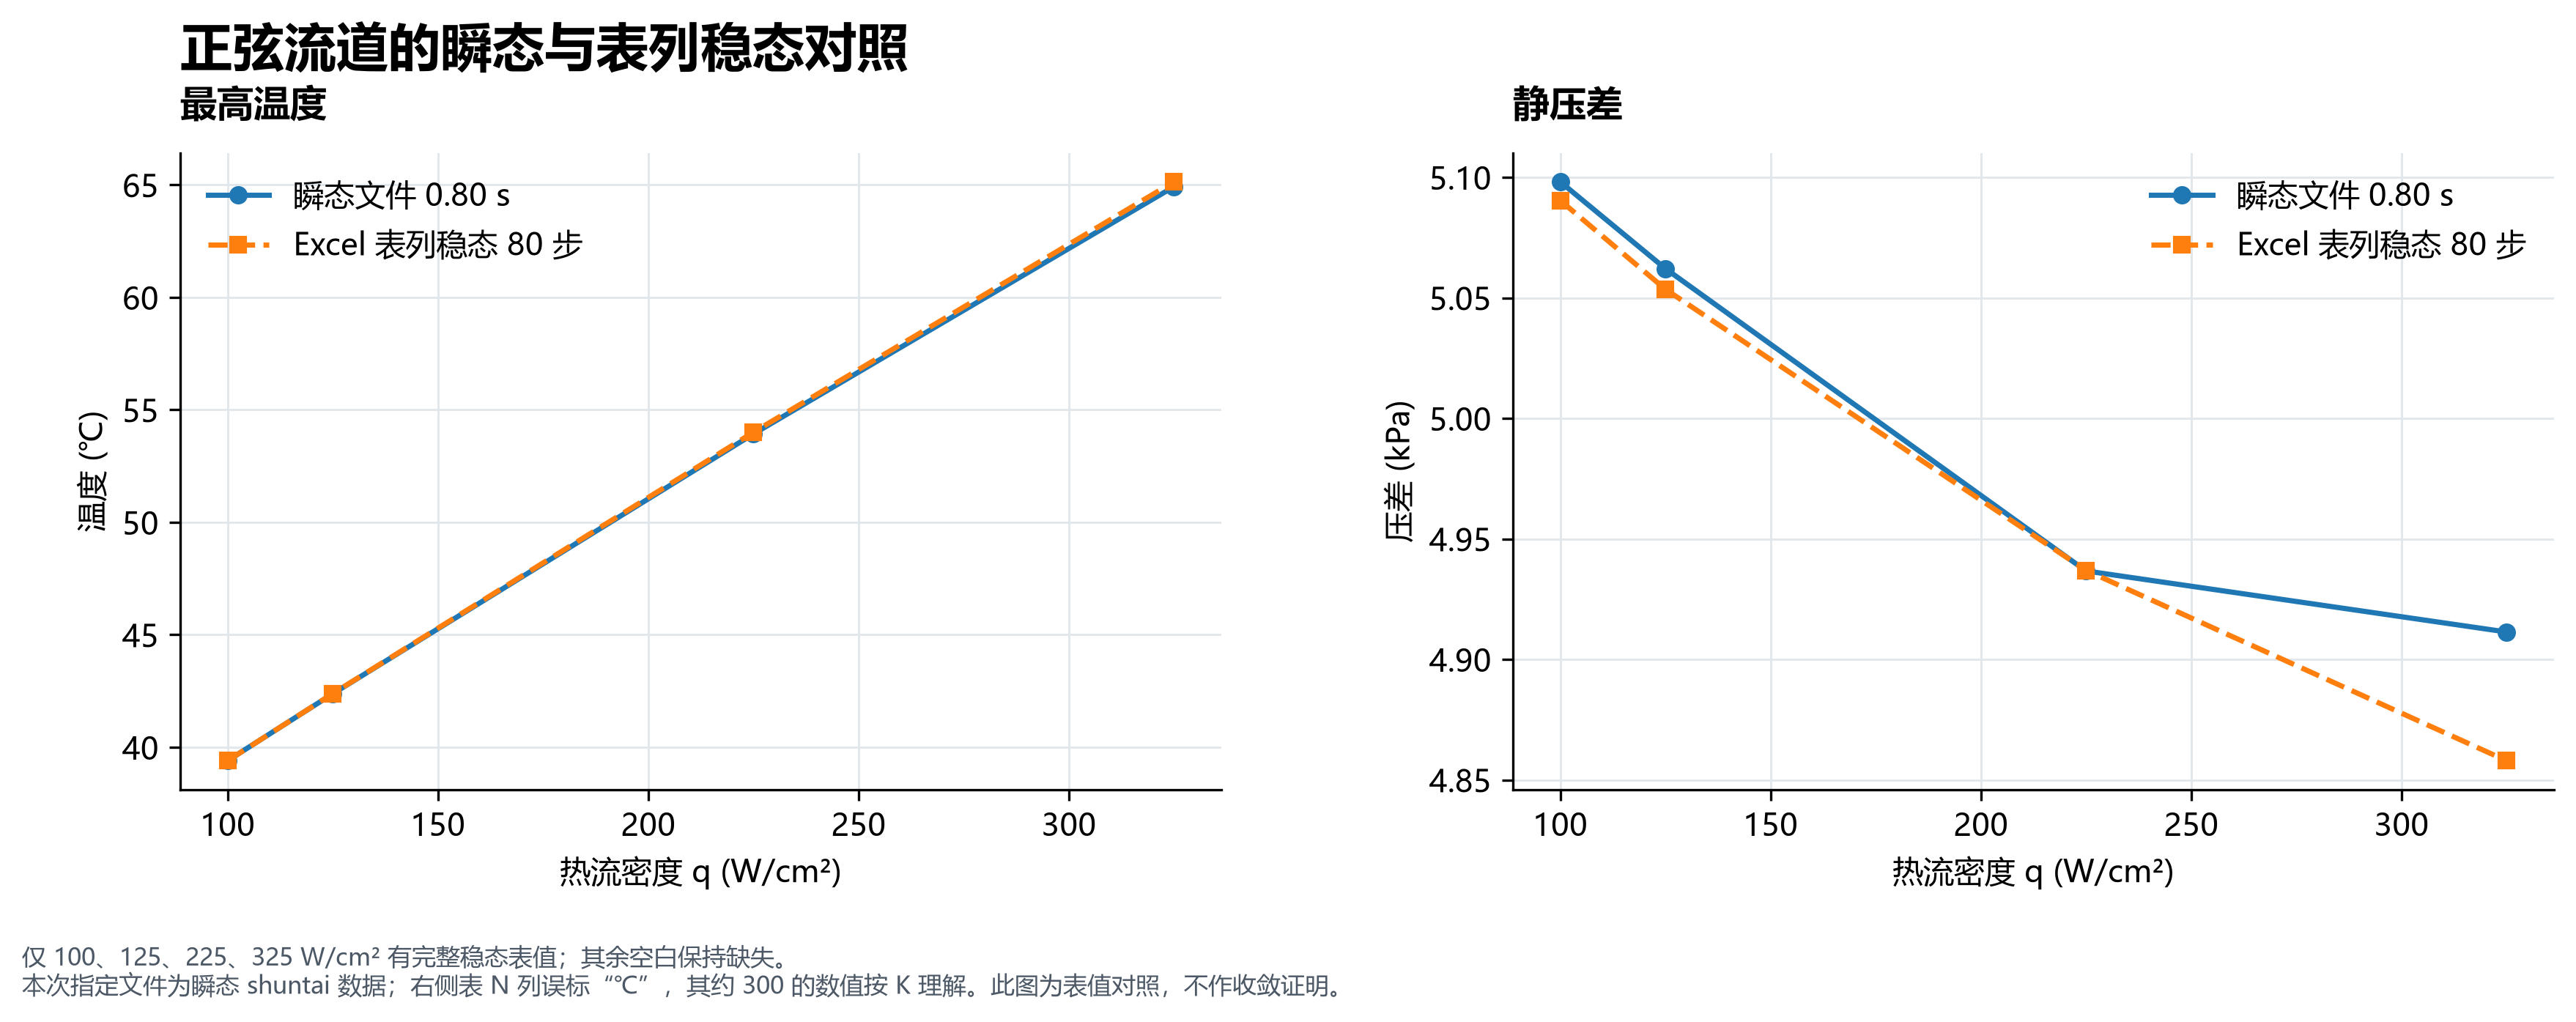
\includegraphics[width=\textwidth]{figs/35_正弦稳态对照.png}
\caption{正弦流道瞬态文件（0.80 s）与表列稳态结果的对照：最高温度与静压差。}
\label{fig:month4-sin-steady}
\end{figure}

数据之间的一致性也做了核对。39 个工况的最高温度与 Data 文件相比偏差不超过 0.00005 K，
体积平均温度不超过 0.00015 K，出口面积平均温度不超过 0.00005 K，
压差落在表值舍入精度内（直线 100 点约 0.50 Pa，合 0.015\%）。
图~\ref{fig:month4-sin-steady} 把正弦的瞬态保存值与表列稳态值叠在一起，
最高温度在四个点上重合，压差的差异不超过 0.05 kPa，属瞬态与稳态的正常差别。
文件、表格与曲线三者的数值互相一致，上述排序不因数据来源而改变。

\textbf{结论。}四种流道的定位可以明确为三条：

\begin{enumerate}
	\item \textbf{中低热流密度下，直线与正弦性能较好。}
	150--300 W/cm$^2$ 区间内两者的最高温度分别为 52.50 与 62.27 $^\circ$C，
	都在 80 $^\circ$C 以内，压差只有 gao2.1 的四分之一左右，
	适合作为该区间承担温度控制的结构。
	\item \textbf{NACA2416 的压降控制最好，适合中低热流密度下以减少压降为目标时采用。}
	其压差为直线的 31.8\%、正弦的 19.9\%，水力功率同样最低；
	代价是最高温度升到 72.48 $^\circ$C，仍在温度余量之内，
	因此在中低热流密度、泵功受限的场合它是最合适的选择。
	\item \textbf{gao2.1 适合高热流密度下的应对与处理。}
	500--1050 W/cm$^2$ 的覆盖范围、1050 点 110.36 $^\circ$C 的最高温度，
	使它成为 500 W/cm$^2$ 以上区间的主力方案：其余三者的已算上限分别止于
	325、325、500 W/cm$^2$；
	代价是压差与水力功率最高，需要用泵功换温度上限。
\end{enumerate}

这三种定位与图~\ref{fig:month4-trend}--图~\ref{fig:month4-sin-steady} 的曲线、
表~\ref{tab:month4-conditions}、表~\ref{tab:month4-advice} 的数值完全一致，
也与月二保存记录的排序一致。

\subsection{可以确定的}

小块分界线研究应由约束条件和性能对照支撑；复杂结构不能凭形态获得优先级；数量与面积需与翼型形状效应区分。

\subsection{尚不能确定的}

各小块交界热流密度、Bi 适用性、扰流柱数量的定量贡献及 XGBoost 性能均待补证据。

\section{问题与初步对策}

\subsection{与预期的差异}

由结构探索转向适用边界研究后，不能再沿用“更复杂即更优”的直观判断。实际需要同时检查导热、对流、水力代价和数量变化。现有非统一工况结果不足以把上述因素分离，理论解释需与后续数据共同修正。



\subsection{遇到的主要问题}

热流密度分界数据、Bi 定义及数量对照尚未齐备；翼型参数组数据不足，XGBoost 暂不具备训练依据。

\subsection{已尝试的方案}

从已有温度与水力记录中提出复杂性问题，并将形状、数量、面积及工况分别记录，形成后续对照要求。

\subsection{下一步对策}

补齐统一工况扫描，验证 Bi 与数量效应；按分组整理数据后开展基础回归与 XGBoost。将得到的小块候选及其条件限制交给逻辑月五整板尝试。

\section{下个月计划}

\begin{table}[H]\centering
\caption{后续工作及所需产出}\label{tab:plan}
\begin{tabularx}{\textwidth}{@{}Y Y Y@{}}
\toprule
\rowcolor{ydzjlight} 工作 & 状态 & 依据或缺口 \\
\midrule
补充理论迭代证据 & 分界线、Bi 与数量对照 & 持续补充 \\
补齐分组并尝试代理模型 & 训练记录及独立测试 & 具备数据后 \\
将局部研究接入整板 & 候选布局、连接和供液条件 & 逻辑月五 \\
\bottomrule\end{tabularx}\end{table}

\FloatBarrier
\Needspace{12\baselineskip}
\begin{thebibliography}{9}
\bibitem{proposal} 大创项目申报书：研究内容与实施方案. 2026.
\bibitem{udf} 项目组. water\_properties\_refprop\_fit.c：液态水物性拟合与 Fluent UDF 源码. 项目计算资料, 2026.
\bibitem{data} 四种流道数据与折线图. 项目计算资料, 2026.
\end{thebibliography}

\end{document}
